%!TEX root = thesis.tex
% Start of content
\chapter{Literature Review}
\label{sec:litrev}

To lay the ground work and context of this research project, this chapter goes into detail on existing
research and work done in the areas of big data processing. Both more traditional batch processing of big
data will be looked at, along with newer advances in the area of realtime stream processing. Different
technologies enabling these processes will be discussed in detail, with the main focus being placed on the
widely used open-source big data projects, such as those encompassed within the Hadoop ecosystem.

The realtime data processing of big data is now of more great importance to both academia and industry than it has
ever been before. Advancements and progress in modern society can be directly attributed back to data and
how we deal with it. The value of data has become increasingly more apparent, and data has become a sort of
currency for the information economy~\cite{st2009examining}. Hence, those in society who realised the value of
data early hold immense power over the entire economy, and in turn society,
overall~\cite{lievesley1993increasing}. From seemingly inconsequential gains at the micro level, such as the
ability to more accurately predict the rise and fall of airline tickets~\cite{darlin2006airfares}, to those
of utmost importance for society as a whole, such as the prediction and tracking of the spread of the Swine Flu
Pandemic in 2009 more accurately than the United States Centers for Disease Control and Prevention
could using big data processing~\cite{ritterman2009using,mayer2013big}. It is applications of big data
processing such as these that have been recognised by academics and organisations in industry alike, with the
last decade seeing a major shift in research and development into new methods for the handling
and processing of big data.

This review will be structured in two main sections.
In~\sectref{sub:batch_data_processing}, an overview and history for the existing major open-source batch
processing systems for big data will be given. This will mostly surround the projects which fall under the
umbrella of the Hadoop ecosystem. In~\sectref{sub:realtime_data_processing}, the current state of realtime
data processing systems for big data will be discussed, including examples of the most widely used open-source realtime
data stream processing systems (DSPS). Comparisons will be drawn between the DSPS technologies and outlined
in how they differ. Further discussion and analysis will be given in~\sectref{sub:processing_conclusion},
including identifying the gaps in existing literature of which this research project aims to fill,
before concluding in~\sectref{sec:conclusion}.

% section introduction (end)


\section{Big Data Processing Background} % (fold)
\label{sec:big_data_processing_background}

Much work has been done in the area of big data processing in the past decade, given the rise of large
scale applications and services, a lot of the time involving large numbers of users and their given data.
Data processing in general has been of large importance for many years, as no matter the business model,
some sort of data has had to be dealt with. Traditionally, this has often been handled through the use of
the relational model, as introduced by Codd~\cite{codd1970relational}. This has been done through the use of relational database
management systems (RDBMS), providing methods for the long term storage of
data and functions for performing queries and manipulation on that data~\cite{astrahan1976system},
such as through use of an implementation of structured query language (SQL)~\cite{chamberlin1974sequel}.

Given larger scales of data in newer projects, along with the needs to scale horizontally in terms of
parallel and distributed processing, the more traditional relational forms of data management have become
less attractive due to their complexity in terms of horizontal scaling~\cite{agrawal2011big}. Hence,
companies dealing with these large scale use cases have started to look outwards to new directions of
data management. This unattractiveness of existing technologies, in terms of scaling and parallelism,
arguably led to the need to develop something new with these objectives in mind.

Note that in this chapter, we will refer to the processing of data in realtime as simply ``realtime data
processing''. This term should be assumed to encompass the meanings that are also often represented through
use of terms such as ``data stream processing'', ``realtime stream processing'', and ``stream processing''.


\section{Batch Data Processing} % (fold)
\label{sub:batch_data_processing}

Over the last decade, the main ``go-to'' solution for any sort of processing needed on datasets falling under
the umbrella of big data has been the MapReduce programming model on top of some sort of scalable distributed
storage system~\cite{bifet_mining_2013}. From a overly simplified functional standpoint, the MapReduce
programming model essentially combines the common \textbf{map} and \textbf{reduce} functions (among others),
often found in the standard libraries of many functional programming languages, such as
Haskell~\cite{lammel2008google}, Clojure~\cite{hickey2008clojure}, or even Java 8~\cite{su2014changing}, to
apply a specified type of processing in a highly parallelised and distributed fashion~\cite{yang2007map}.

The MapReduce data processing model specialises in batch mode processing on data which is already available.
Batch data processing can be thought of where data needed to be processed is first queued up in ``batches''
Once ready, those batches get fed into the processing system and handled accordingly~\cite{condie2010online}.


\subsection{MapReduce and GFS} % (fold)
\label{ssub:mapreduce_and_gfs}

Dean and Ghemawat, in~\cite{dean_mapreduce:_2008}, originally presented MapReduce as a technology that had been
developed internally at Google, Inc.\ to be an abstraction to simplify the various computations that engineers were
trying to perform on their large datasets. The implementations of these computations, while not complicated functions
themselves, were obfuscated by the fact of having to manually parallelise the computations, distribute the data, and
handle faults all in an effective manner that met their performance requirements. The MapReduce model that was developed,
enabled these computations to be approached from a more simple, high-level manner without the programmer needing to worry
about optimising for available resources. In this way, it was more ``declarative'' while still allowing it to be written
in a procedural language, such as Java. Furthermore, the MapReduce abstraction provided high horizontal scalability to
differently sized clusters running on modest hardware.

While MapReduce conceptually offers many features that may be found in parallel database technologies, Dean and
Ghemawat, in~\cite{dean2010mapreduce}, emphasise the differences, and specifically flawed assumptions made about MapReduce
in light of parallel databases. Issues in parallel databases such as fault tolerance when it comes to job failure,
difficulties with input data from heterogeneous sources, and performing more complicated functions than those supported
in SQL, are all fully supported and taken into consideration with MapReduce. Notably, while the programming model
allows for further complicated functions, it also remains to be simple with only two major functions that need to be
implemented: \textbf{map} and \textbf{reduce}~\cite{pavlo2009comparison}.

As previously stated, the MapReduce programming model is generally used on top of some sort of distributed storage
system. In the previous case at Google, Inc., in the original MapReduce implementation, it was implemented on top of
their own proprietary distributed file system, known as Google File System (GFS). Ghemawat et al.,
in~\cite{ghemawat_google_2003}, define GFS to be a ``scalable distributed file system for large distributed data-intensive
applications'', noting that can be run on ``inexpensive commodity hardware''. Note that GFS was designed and in-use
at Google, Inc.\ years before they managed to develop their MapReduce abstraction, and the original paper on MapReduce
from Dean and Ghemawat state that GFS was used to manage data and store data from MapReduce~\cite{dean_mapreduce:_2008}.
Furthermore, McKusick and Quinlan, in~\cite{mckusick2009gfs}, state that, as of 2009, the majority of Google's data
relating to their many web-oriented applications rely on GFS.

% subsubsection mapreduce_and_gfs (end)


\subsection{Hadoop MapReduce and HDFS} % (fold)
\label{ssub:hadoop_mapreduce_and_hdfs}

While MapReduce paired with GFS proved to be very successful solution for big data processing at Google, Inc., and
there was a considerable amount of notable research published on the technology, it was proprietary in-house software
unique to Google, and availability elsewhere was often not an option~\cite{grossman2009varieties}. Hence, the
open-source software community responded in turn with their own implementation of Google's MapReduce and a
distributed file system on which it runs,
analogous to the role GFS played. The file system is known as the Hadoop Distributed File System (HDFS). Both of these
projects, along with many others to date, make up the Apache Hadoop
big data ecosystem. The Apache Hadoop ecosystem, being a top level Apache Software
Foundation open-source project, has been developed by a number of joint contributors from various organisations and
institutions such as Yahoo!, Inc., Intel, IBM, UC Berkeley, among others~\cite{hadoop_committers}.

While Hadoop's MapReduce implementation very much was designed to be a complete functional replacement for Google's MapReduce, based upon published works by Google,
HDFS is an entirely separate project in its own right. In the original paper from Yahoo!~\cite{shvachko_hadoop_2010},
Inc., Shvachko et al.\ present HDFS as ``the file system component of Hadoop'' with the intention of being similar to
in external appearance to the UNIX file system, however they also state that ``faithfulness to standards was sacrificed
in favour of improved performance''.

While HDFS was designed with replicating GFS' functionality in mind, several low-level architectural and design decisions
were made that substantially differ to those documented in GFS. For example, in~\cite{borthakur2007hadoop}, Borthakur
documents the method HDFS uses when it comes to file deletion. Borthakur talks about how when a file is deleted in HDFS,
it essentially gets moved to a \texttt{/trash} directory, much like what happens in a lot of modern operating systems.
This \texttt{/trash} directory is then purged after a configurable amount of time, the default of which being six hours.
To contrast with this, GFS is documented to have a more primitive way of managing deleted files. Ghemawat, et al.,
in~\cite{ghemawat_google_2003}, document GFS' garbage collection implementation. Instead of having a centralised
\texttt{/trash} storage, deleted files get renamed to a hidden name. The GFS master then, during a regularly scheduled
scan, will delete any of these hidden files that have remained deleted for a configurable amount of time, the default
being three days. This is by far not the only difference between the two file systems, this is simply an example of a
less low-level technical difference.

HDFS, being designed as a standalone technology, is now used as a data storage component for many different big data
technologies, not limited to only those within the Hadoop ecosystem~\cite{taylor2010overview} but also projects
outside~\cite{xin2013graphx,yang2013big}. HDFS was designed with general usage in mind and designed with horizontal
scalability being a key consideration, hence runs on inexpensive clusters using modest hardware, while still delivering all
its potential advantages~\cite{borthakur2008hdfs}.

% subsubsection hadoop_mapreduce_and_hdfs (end)


\subsection{Pig and Hive} % (fold)
\label{ssub:pig_and_hive}

Given the popularity of Hadoop, there were several early attempts at building further abstractions on top of the
MapReduce model, which were met with a high level of success. As highlighted earlier, MapReduce was originally designed
to be a nice abstraction on top of the underlying hardware, however according to Thusoo et al., in~\cite{thusoo2009hive},
MapReduce was still too low level resulting in programmers writing programs that are considered to be ``hard to maintain
and reuse''. Thus, Thusoo et al., at Facebook Inc., built the Hive abstraction on top of MapReduce. Hive allows
programmers to write queries in a similarly declarative language to SQL --- known affectionately as \textit{HiveQL} ---
which then get compiled down into MapReduce jobs to run on Hadoop~\cite{thusoo2010hive}.

Hive, along with HiveQL, provide a platform to run ad-hoc queries on top of HDFS stored data, which are run as batch
MapReduce jobs. For example, all generated reports on Facebook to their paid advertisers are generated using batch jobs
constructed using Hive, along with several other analytics use cases at Facebook~\cite{thusoo2010data}. An added benefit
shown at Facebook from the use of Hive, over traditional MapReduce, was the users familiarity with SQL-like
declarativeness in regards to querying and manipulating data~\cite{borthakur2011apache}.

Another commonly used abstraction, that was developed prior to Hive, was what is known simply as Pig. Like Hive, Pig attempts to
be a further higher level abstraction on top of the MapReduce model, which ultimately compiles down into MapReduce jobs.
what differentiates it more from Hive is that instead of offering a solely declarative SQL-like language for data
manipulation and querying, it offers a language that takes more of a procedural and functional dataflow paradigm
influenced approach~\cite{olston2011nova}. This still allows for relational algebraic constraints to be specified on the data set in relation to defining the
result~\cite{olston_pig_2008}. Olston et al.\ describe Pig's language --- known as \textit{Pig Latin} --- to be what they
define as a ``dataflow language'', rather than a strictly procedural or declarative language.

Pig works by having the program first parsed into a directed acyclic graph (DAG), which then can be be optimised using
DAG-related graph theory operations, before having that DAG being compiled down into native MapReduce batch jobs. The MapReduce
stage is also optimised through use of function ordering, before being submitted to run on a Hadoop
cluster~\cite{stewart2011comparing}.

Hive, also being a high level abstraction on top of MapReduce, also enable many of their own
optimisations to be applied to the underlying MapReduce jobs during the compilation
stage~\cite{gates2009building,thusoo2010hive} as well as having the benefit of being susceptible to manual query
optimisations, familiar to programmers familiar with query optimisations from SQL~\cite{gruenheid2011query}.

% subsubsection pig_and_hive (end)

% subsection batch_data_processing (end)




\section{Realtime Data Processing} % (fold)
\label{sub:realtime_data_processing}

With HDFS being an open-source project, with a large range of users~\cite{hadoop_users} and code
contributors~\cite{hadoop_committers}, it has grown as a project in the last few years for uses beyond what it was
originally intended for: a backend storage system for Hadoop MapReduce. HDFS is now not only used with Hadoop's
MapReduce, but also with a variety of other technologies, a lot of which run as a part of the Hadoop ecosystem, but
also those which do not.
Big data processing has moved on from the more ``traditional'' method of processing, involving MapReduce jobs, which
were most suitable for the batch processing of data, to those methods which specialise in the realtime processing of
streamed data.
The main difference of which is that rather than waiting for all the data before processing can be started, in realtime
data processing, the data can be streamed into the processing system and processed at any time with whatever data is
made available.

The use cases for such realtime data processing differ much from batched processing in ways a lot of the time relating
to the availability of data. With batch jobs, generally processing is done after-the-fact, or after data has been
collected from various sources and stored in a system, similar to HDFS. With realtime data processing, data can be
processed as soon as it is received from sources, without using a storage system, such as HDFS, to first hold it.
For example, an array of sensors can stream their data directly to the data stream processing system (DSPS), without
any intermediate step. From there, the DSPS will process the data according to how it is programmed, and either
send it on to further systems, or store it for later batch processing.


\subsection{Hadoop YARN} % (fold)
\label{ssub:apache_hadoop_yarn_}

As previously looked at, the aim of the MapReduce model was performing distributed and highly parallelised computations
on distributed batches of data. This suited a lot of the big data audience, and hence Hadoop became the dominant
method of big data processing for many years~\cite{liu_survey_2014}. However for some more specialised applications, such as
the realtime monitoring of sensors, as touched on earlier, stock trading, and realtime web traffic analytics, the high
latency between the data arriving and actual results being generated from the computations was not
satisfactory~\cite{kamburugamuve_survey_2014}. Furthermore, such use-cases were simply not suited for batch processing.

A recent (2013) industry survey on European company use of big data technology by Bange, Grosser, and Janoschek, noted
in~\cite{industry_bd_survey}, shows that over 70\% of responders show a need for realtime processing. In that time,
there has certainly been a response from the open-source software community, responding with extensions to more
traditional batch systems, such as Hadoop MapReduce, along with complete standalone DSPS solutions.

On the Hadoop front, the limitations of the MapReduce model were recognised, and a large effort was made in developing
the ``next generation'' of Hadoop so that it could be properly extensible and used with other programming models not locked into
the rigidity of the MapReduce model. This change in Hadoop became known officially known as YARN (Yet Another Resource Negotiator). According to
the original developers of YARN, Vavilapalli et al.\ state that YARN enables Hadoop to become more modular, decoupling
the resource management functionality of Hadoop from the programming model (traditionally,
MapReduce)~\cite{vavilapalli_apache_2013}.
For Hadoop end-users, this decoupling essentially allowed for non-MapReduce technologies to be built on top of the Hadoop
ecosystem, which was traditionally a part of MapReduce, allowing for much more flexible applications of big data
processing on top of the existing robust framework Hadoop provides.

Examples of such systems now built, or in some cases ported, to run on top of Hadoop, providing alternative processing
applications and use cases, include:

\begin{itemize}
  \item Dryad, a general-purpose distributed execution system from Microsoft Research~\cite{isard2007dryad}. Dryad is
  aimed at being high level enough to make it easy for developers to write highly distributed and parallel applications.
  \item Spark, a data processing system, from researchers at UC Berkeley, that focuses on computations that reuse the
  same working data set in-memory over multiple parallel operations~\cite{zaharia2010spark}. Spark, and in particular Spark
  Streaming, will be looked at further in~\sectref{ssub:spark_streaming}.
  \item Storm, a realtime stream processing system~\cite[p.\ 244]{murthy2013apache}. Storm allows specified processing
  on an incoming stream of data indefinitely, until stopped. Storm will be looked at further in~\sectref{ssub:storm}.
  \item Tez, an extensible framework which allows for the building of batch and interactive Hadoop
  applications~\cite{web_tez}.
  \item REEF, a YARN-based runtime environment framework~\cite{chun2013reef}. REEF is essentially a further abstraction
  on top of YARN, with the intention of making a unified big data application server.
  \item Samza, a relatively new realtime data processing framework from LinkedIn. Discussed further in~\sectref{ssub:samza}.
\end{itemize}

These are just some of the more popular examples of applications built to interact with the Hadoop ecosystem via YARN.

With the emergence of YARN, the ability to build DSPS technologies on top of Hadoop led to a lot of interest in realtime
processing solutions that was often looked over by previous Hadoop batch users.

% subsubsection apache_hadoop_yarn_ (end)


\subsection{Storm} % (fold)
\label{ssub:storm}

One very notable DSPS technology developed independently of Hadoop, and that is gaining immense popularity and growth in its
user base, is the Storm project. Storm was originally developed by a team of engineers lead by Nathan Marz at
BackType~\cite{web_storm}. BackType has since been acquired by Twitter, Inc.\ where development has
continued. Toshniwal et al.~\cite{toshniwal_stormtwitter_2014}\ describe Storm, in the context of its use at Twitter, as ``a
realtime distributed stream data processing engine'' that ``powers the real-time stream data management tasks that are
crucial to provide Twitter services''~\cite[p.\ 147]{toshniwal_stormtwitter_2014}. Since the project's inception, Storm has seen mass
adoption in industry, including amongst some of the biggest names, such as Twitter, Yahoo!, Alibaba, and
Baidu~\cite{storm_users}.

While Storm does not run on top of YARN, there is currently a large effort from engineers at Yahoo!, Inc.\ being put
into a YARN port for Storm, aptly named \textit{storm-yarn}~\cite{web_storm_yarn,kumar2014architectural}. This YARN port will
allow applications written for Storm to take advantage of the resources managed in a Hadoop cluster by YARN. While still
in early stages of development, storm-yarn has begun to gain attention in the developer community, through focus from
channels such as the Yahoo Developer Network~\cite{web_yahoo_blog} and Hortonworks~\cite{web_hortonworks_blog}.

The programming model for Storm consists of a Storm topology. This topology is made up of various components, which
either ``transform'' the data in some specified way (known as a \textit{bolt}), or input the data from a specified source
before outputting it to one of the given bolts (known as a \textit{spout}). The layout of spouts and bolts are then
constructed in a separate topology definition, defining the way the data streams (represented as tuples) flow through
the topology~\cite{jones2013process}. An example Storm topology is shown in~\figref{fig:storm_topology}.

\begin{figure}[ht]
  \centering
  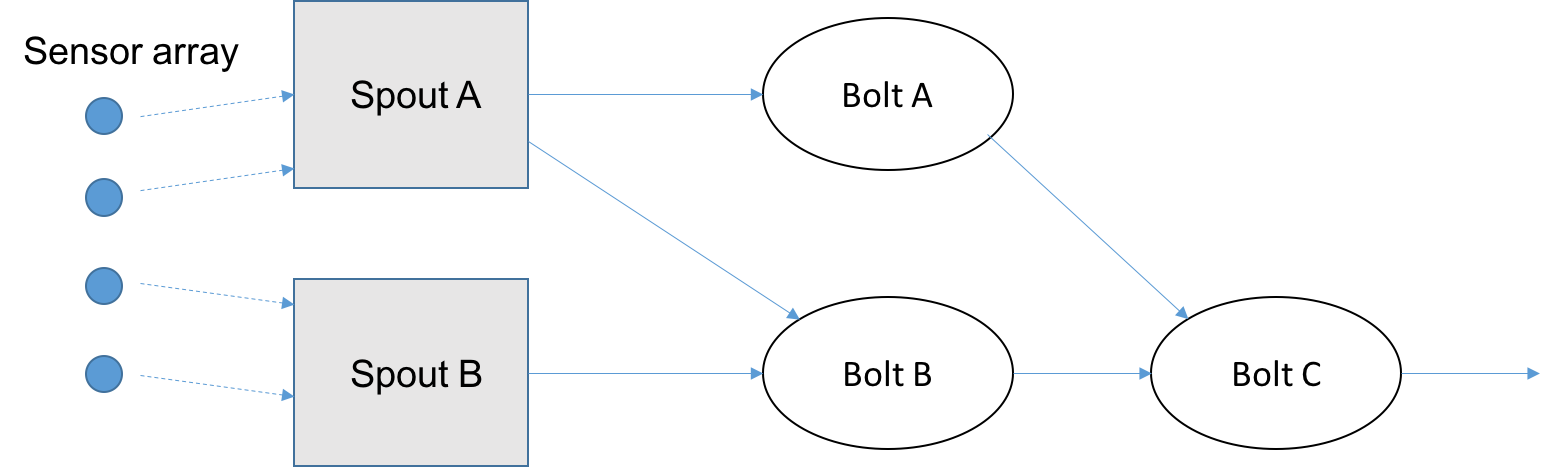
\includegraphics[width=0.8\textwidth]{includes/figures/fig_storm_topology1}
  \caption{An example Storm topology showing the source of the tuple stream from spouts A and B, received from an array
  of sensors, which then forwards the stream on for processing at bolts A and B. Bolts can forward streams
  onto other bolts.}
  \label{fig:storm_topology}
\end{figure}

Storm, while predominantly written in Clojure, running on the JVM, allows topologies to be defined and written in any
available programming language through the use of a Thrift definition for topologies~\cite{About8:online}. Thrift is
a software library, developed at Facebook, Inc., for the purpose of defining datatypes and interfaces for use in
multiple programming languages~\cite{slee2007thrift}. Storm provide example Storm projects written in Java, Clojure,
and Python, however most official Storm documentation, at present, use Java.

% subsubsection storm (end)


\subsection{Spark StreaminS} % (fold)
\label{ssub:spark_streaming}

Spark is another popular big data distributed processing framework, offering of both realtime data processing
and more traditional batch mode processing, running on top of YARN~\cite{zaharia2010spark}. Spark was developed at UC
Berkeley, and is notable for its novel approach to in-memory computation, through Spark's main data abstraction which is
termed a \textit{resilient distributed dataset} (RDD). An RDD is a set of data on which computations will be performed,
which can be specified to be cached in volatile memory across multiple machines. What this then allows is multiple
distributed operations being performed on this same dataset in parallel without such overhead, as secondary storage
IO operations, which is noted by Spark as a performance limitation of MapReduce~\cite{davidson2013optimizing}. Spark is designed with highly iterative
computations in-mind.

The Spark project has experienced a large growth in terms of project contributions over the past few years, now
encompassing a number of sub-projects running on top of the Spark engine, all suited for different use cases. These
include:

\begin{itemize}
  \item \textbf{Spark SQL}: An SQL-like engine that runs on top of Spark,
  allowing Spark users to reap the benefits of using a declarative SQL-like language on top of Spark's functional
  API~\cite{armbrustspark}. (Previously known as Shark~\cite{xin2013shark}).
  \item \textbf{Spark GraphX}: A graph abstraction on top of the Spark engine, allowing for the efficient expression of
  distributed graph structures and computations on those structures~\cite{xin2013graphx}.
  \item \textbf{Spark MLlib}: A distributed scalable machine learning platform on top of Spark, allowing for efficient
  machine learning capabilities~\cite{sparks2013mli}.
  \item \textbf{Spark Streaming}: A DSPS platform built on top of the Spark engine, allowing for the processing of data
  in realtime~\cite{zaharia2012discretized}.
\end{itemize}

Given these different platforms built on top of Spark's in-memory computation engine, Spark offers solutions for many
different big data processing use cases. We are most interested in Spark Streaming, given its realtime DSPS offerings.
Spark Streaming uses a different programming model than that which is offered in the base Spark platform, that involves what
is labelled as \textit{DStreams} (discretised streams). DStreams essentially allows for a series of deterministic batch computations
be treated as single a realtime data stream~\cite{zaharia2012discretized}. The DStream model is specific to the Spark Streaming
system --- the original batch mode Spark system continues to use the previously mentioned RDD abstraction --- and the
creators claim performance improvements of being $2-5\times$ faster than other DSPS technologies, such as S4
and Storm, given its use of in-memory stream computation~\cite{zaharia2013discretized}. However, this is a topic of debate,
with opponents claiming that these Spark performance claims are very much dependent on external factors, such as
available system resources~\cite{web_slideshare_b}.

Both Spark and Spark Streaming have started to gain notable usage in both industry and research projects in academia in
the last few years. Online video distribution company, Conviva Inc., report to be using Spark for the processing of
analytics reports, such as viewer geographical distribution reports~\cite{web_spark_conviva,zaharia2012fast}. The Mobile
Millennium project at UC Berkeley~\cite{web_spark_mmp}, a traffic monitoring system that uses GPS through users'
cellular phones for traffic monitoring in the San Francisco Bay Area, has been using Spark for scaling the main
algorithm in use for the project: an expectation maximisation (EM) algorithm that has been parallelised by being run on
Spark~\cite{hunter2011scaling}.

Spark Streaming, while originally written in Scala, supports official APIs for Java, Scala, and Python. Note that the
Python API for Spark has only recently been introduced and, as of yet (version 1.3.1), does have have support for all
the data sources which Java and Scala offer~\cite{Spark5:online}.

% subsubsection spark_streaming (end)


\subsection{Samza} % (fold
\label{ssub:samza}

Samza is a relatively new realtime big data processing framework originally developed in-house at LinkedIn, which has since been
open-sourced at the Apache Software Foundation~\cite{web_samza}. Samza offers much similar functionality to that of
Storm, however instead the running of Samza is highly coupled with the Kafka message broker, which handles the input
and output of data streams. Essentially, Kafka is a highly distributed messaging system that focusses on the handling
of log data~\cite{kreps2011kafka}, integrating with the Hadoop ecosystem.

While Samza is lacking in maturity and adoption rates, as compared to projects such as Storm, it is built on mature
components, such as YARN and Kafka, and thus a lot of crucial features are offloaded onto these platforms. For example,
the archiving of data, stream persistence, and imperfection handling is offloaded to Kafka~\cite{bockermann2014survey}.
Likewise, YARN is used for ensuring fault tolerance through the handling of restarting machines that have failed in a
cluster, among further resource management~\cite{bockermann2014survey}.

Samza processes streams of data through pre-defined jobs which perform any specified operation on the data streams, much
like bolts in Storm. The source of streams in Samza comes from Kafka, which can be also used as an output destination
for jobs. How the data is received from the actual source (such as a sensor), then sent through Kafka is a matter of
further implementation on the part of the programmer~\cite{yangradstack}. Note that a layout of jobs in Samza differs considerably from defining
a Storm topology layout, in that each individual job defines its input and output sources, rather than jobs being
linked together in a separate definition file.

Samza is mainly programmed using Scala, running on the JVM, and allows programming of jobs through a set of Java
interfaces~\cite{Samza6:online}. It is officially supported and recommended to program Samza jobs in Java, however it
would also be possible to implement the provided interfaces using any JVM language, such as Scala or Clojure.

% subsubsection samza (end)


\subsection{S4} % (fold)
\label{ssub:s4}

S4 (Simple Scalable Streaming System) is another realtime big data processing framework that originated at Yahoo!, Inc.\
that has since been open-sourced~\cite{neumeyer2010s4}. It is a relatively old project compared to the before-mentioned
projects, with development becoming less of a priority in the last few years, with the last update being released in 2013.
S4 was highly influenced in design by the MapReduce programming model.

Much like what was noted about Samza in~\sectref{ssub:samza}, S4 attempts offload several lower level tasks to more
mature and established systems specialising in those areas. The logical architecture of S4 lays out its jobs in a
network of processing elements (PEs) which are arranged as a directed acyclic graph. Each of these PEs entail the type
of processing to be done on the data at that point in the network. Each of the PEs are assigned to a processing node, a
logical host in the cluster. The management and coordination of these processing nodes is offloaded by S4 to
ZooKeeper~\cite{kamburugamuve_survey_2014}. Much like the before-mentioned Kafka, ZooKeeper in itself is its own complex
service used as a part of many different big data infrastructures, including Samza. ZooKeeper specialises in the
high-performance coordination of distributed processes inside distributed applications~\cite{hunt2010zookeeper}.

Note that a number of performance issues have been noted in S4, including non-linear performance scalability, bad
resource management, low expectations on fault tolerance, and high reliance on the network~\cite{chauhan2012performance}.
As mentioned earlier, development on S4 has stagnated. Adoption of S4 over DSPS platforms, such as Samza, Storm,
and Spark Streaming, has not been seen to be major, and literature in big data research have shown a significant lack of
focus on S4 when looking at the topics of DSPS technologies.

% subsubsection s4 (end)

% subsection realtime_data_processing (end)


\section{Discussion and Analysis} % (fold)
\label{sub:processing_conclusion}

From the previously covered literature, it is rather difficult to provide a reasonable comparison for all the different
realtime data processing projects. A lot of the claims made in original literature relating to the projects cannot be
quantified impartially, as comparisons or tests have not been carried out relating to other projects. Instead, Stonebraker,
\c{C}\~entintemel, and Zdonik proposed what they claim to be the eight requirements for realtime data processing systems~\cite{stonebraker_8_2005},
which can be used to given an impartial comparison of the previously covered projects. The requirements were defined a
number of years prior to the creation of the four main realtime data processing systems that were covered (2005), however are highly
cited as being the defining features that the current generation of realtime data processing systems have strived to meet.
The requirements, put forward by Stonebraker et al., are summarised as follows:

\noindent \textbf{1: Keep the data moving -} This requirement relates to the high mobility of data and importance of low
latency in the overall processing. Hence, processing should happen as data moves, rather than storing it first then
processing what is stored.

\noindent \textbf{2: SQL on streams -} This requirement states that a high-level SQL-like query language should be
available for performing on-the-fly queries on data streams. SQL is given as an example, however it is noted the language's
operators should be more oriented to data streams.

\noindent \textbf{3: Handle stream imperfections -} Given the high degree of imperfections in data streams, including
factors such as missing and out-of-order data, this requirement states that processing systems need to be able to handle
these issues. Simply waiting for all data to arrive if some is missing is not acceptable.

\noindent \textbf{4: Generate predictable outcomes -} This requirement relates to the determinism associated with the
outcomes of specified processes to be applied to data. A realtime processing system should have predictable and repeatable
outcomes. Note that this requirement is rather hard to satisfy as in practice data streams are, by character, rather
unpredictable. However, the operations performed on given data, and thus the outputs, are required to be predictable.

\noindent \textbf{5: Integrate stored and streamed data -} This requirement states that a realtime processing system
should provide the capabilities to be able to process both data that is already stored and data that is being delivered
in realtime. This should happen seamlessly and provide the same programming interface for either source of data.

\noindent \textbf{6: Guarantee data safety and availability -} This requirement states that realtime processing systems
should ensure that they have a high level of availability for processing data, and in any cases of failures, the integrity
of data should remain consistent.

\noindent \textbf{7: Partition and scale applications automatically -} This requirement states that the partitioning of
and processing of data should be performed transparently and automatically over the hardware on which it is running on.
It should also scale to more different levels of hardware without user intervention.

\noindent \textbf{8: Process and respond instantaneously -} This requirement relates to delivering highly responsive
feedback to end-users, even for high-volume applications.

The previously covered literature has been used to determine whether or not the before-mentioned realtime data processing
systems adhere to these requirements. The outcome of this is shown in~\tabref{tab:processing_systems_compare}.

Note that in~\tabref{tab:processing_systems_compare}, those cells with ``N/A'' as the value simply mean that the literature
is inconclusive on whether or not they adhere to the particular requirement.

\import{includes/tables/}{data_processing_compare}

From this table, we can note that literature covering both deterministic outcomes and instant response from each of the DSPS technologies
are not consistent. This may not be a problem for the project at hand, however proves to be a factor for further research.
Furthermore, the possibility of performing batch computations on stored data are not available on both S4 and Samza. Given
the dominance of batch processing shown to be needed in many areas of big data processing, this would be an important
factor of adoption of DSPS technologies in many existing applications. Existing applications may want to introduce realtime
data processing on-top of their existing batch processing logic. With technologies affording both batch and realtime data processing
possibilities, both Storm and Spark Streaming would be very appealing options.

% subsection conclusion (end)

% section big_data_processing_background (end)


\section{Conclusion} % (fold)
\label{sec:conclusion_litrev}

The choosing of appropriate realtime data processing platforms for the processing of a given application and dataset
is an important, and often confusing, problem. Most platforms compare themselves in terms of performance with other
frameworks, often which are disputed by members in other platform ``camps''~\cite{web_slideshare_b,web_slideshare_a}.
Hence, providing an informed recommendation based on the features each platform offers, and an impartial performance
evaluation is a much needed and important contribution to address this gap in qualitative and quantitative evaluations
of the available platforms. These evaluations will be looked at further in Chapter 4.

From looking at existing literature in the area of realtime data stream processing, we have identified four candidate
data stream processing technologies for use in the evaluation:
\begin{itemize}
  \item Storm
  \item Samza
  \item Spark Streaming
  \item S4
\end{itemize}
However, due to the noted issues in S4 relating to lack of development, lack of adoption, and performance issues, in relevant
literature, we have made the decision to ignore S4 for use in the overall evaluation. Hence, evaluation will be constrained
to the candidate DSPS technologies of Samza, Spark Streaming, and Storm.

This research will further the field of realtime big data processing in addressing these shown gaps, and making the
decision process far more streamlined for researchers and developers of DSPS technologies alike.

% section conclusion (end)

